\documentclass[oneside,12pt,letterpaper]{article}

% Imports and Definitions
%% Packages
\usepackage{amsmath}
\usepackage{amsfonts}
\usepackage{amssymb}
\usepackage{amsthm}
\usepackage{arydshln}
\usepackage{color}
\usepackage{extramarks}
\usepackage{fancyhdr}
\usepackage{float}
\usepackage[margin=1in]{geometry}
\usepackage{graphicx}
\usepackage{listings}
\usepackage{multicol}
\usepackage{setspace}
\usepackage{subcaption}
\usepackage{textcomp}
\usepackage{url}
\usepackage{xspace}
\usepackage{mathtools}

%% Commands
%%% Metadata
\newcommand{\metaTitle}{Comprehensive Exam}
\newcommand{\metaDueDate}{November 24, 2020}
\newcommand{\metaDueTime}{04:00 PM}
\newcommand{\metaSchool}{IUPUI}
\newcommand{\metaClass}{STAT 52400}
\newcommand{\metaDepartment}{Statistics Department}
\newcommand{\metaAuthorName}{Ross Grinvalds}

%%% Aliases
\newcommand{\Bias}{\mathrm{Bias}}
\newcommand{\Cov}{\mathrm{Cov}}
\newcommand{\dd}[1]{\frac{\mathrm{d}}{\mathrm{d}x} (#1)}
\newcommand{\dx}{\mathrm{d}x}
\newcommand{\E}{\mathrm{E}}
\newcommand{\m}[1]{\begin{bmatrix*}[r]#1\end{bmatrix*}}
\newcommand{\md}[1]{\begin{vmatrix*}#1\end{vmatrix*}}
\newcommand{\mf}[1]{\mathrm{\bf{#1}}}
\newcommand{\p}[1]{\begin{pmatrix}#1\end{pmatrix}} 
\newcommand{\pdd}[2]{\frac{\partial}{\partial #1} (#2)}
\newcommand{\solution}{\textbf{\large Solution}}
\newcommand{\T}{\intercal}
\newcommand{\Var}{\mathrm{Var}}

%%% Math Functions
\makeatletter
\newsavebox{\mybox}\newsavebox{\mysim}
\newcommand{\distras}[1]{%
  \savebox{\mybox}{\hbox{\kern3pt$\scriptstyle#1$\kern3pt}}%
  \savebox{\mysim}{\hbox{$\sim$}}%
  \mathbin{\overset{#1}{\kern\z@\resizebox{\wd\mybox}{\ht\mysim}{$\sim$}}}%
}
\makeatother

\newcommand{\indep}{\perp \!\!\! \perp}

%% Environments
%%% R Code
\newcommand{\ri}[1]{\lstinline{#1}}  %% Short for 'R inline'

\lstnewenvironment{rc}[1][]{
	\lstset{commentstyle=\color{red}, keywordstyle=\color{black}, showstringspaces=true, language=R, basicstyle=\ttfamily\tiny}
}{}
\lstset{language=R}


% Settings
%% Document-wide
\pagestyle{fancy}

%% Header and Footer
\setlength{\headheight}{15pt}
\lhead{\metaAuthorName}
\chead{\metaSchool\ \metaClass:\ \metaTitle}
\rhead{\metaDepartment}
\cfoot{\thepage}

%% Title Page
\title{
	\vspace{1in}
	\textmd{\textbf{\metaSchool\ \metaClass:\ \metaTitle}}\\
	\normalsize\vspace{0.1in}\small{Due\ by\ \metaDueDate\ at \metaDueTime}\\
	\vspace{6in}
}
\author{\metaAuthorName}
\date{}


\begin{document}
\maketitle

\section*{Problem 9.19} 
This factor analysis focuses on data collected from a firm that is evaluating the quality of its sales personnel. Included in the variables are a set of three indices that measure sales performance and four test results that measure different capacities of intelligence. A total of $n=50$ observations were collected for the study.

\begin{enumerate}
\item[\bf{a)}]
	An orthogonal factor model generated on $m=2$ and $m=3$ factors. Before the factor analysis was carried out, the data were standardized as follows: $$Z_i = \frac{X_i - \mu_i}{\sqrt{\sigma_{ii}}}$$ The maximum likelihood solutions for $m=2$ were computed in $R$ using the `factanal' function. When the model is fit `orthogonally', it is meant that the factors are not rotated.

\begin{rc}

Call:
factanal(x = Z, factors = 2, rotation = "none")

Uniquenesses:
index_growth     0.069
index_profit     0.070	
index_newsales	 0.123
test_creativity  0.005 
test_mechanical  0.474	
test_abstract	   0.614	
test_mathematics 0.029 

Loadings:
                Factor1 Factor2
index_growth      0.695   0.669 
index_profit      0.669   0.695 
index_newsales    0.795   0.494 
test_creativity   0.983  -0.167 
test_mechanical   0.655   0.312 
test_abstract     0.250   0.569 
test_mathematics  0.558   0.812 

                Factor1 Factor2
SS loadings      3.333   2.283
Proportion Var   0.476   0.326
Cumulative Var   0.476   0.802

Test of the hypothesis that 2 factors are sufficient.
The chi square statistic is 117.2 on 8 degrees of freedom.
The p-value is 1.25e-21 

\end{rc}

	The interpretation of the first component seems to give a general performance index of a sales person. The greater load assigned to creative aptitude suggests the factor explains this variable very well. The second factor does not assign a strong loading to creativity, but increases the loading on abstract and mathematical reasoning. It isn't entirely clear how to interpret the second factor. The overall chi square statistic is formed by a likelihood ratio test. A significant p-value suggests that the factor model approximates the covariance matrix (in this case, correlation matrix) well. The total proportion of variance explained by the model is $80.2\%$

	If a total of $m=3$ factors are considered:

\begin{rc}

Call:
factanal(x = Z, factors = 3, rotation = "none")

Uniquenesses:
index_growth     0.039
index_profit     0.034	
index_newsales	 0.088
test_creativity  0.005 
test_mechanical  0.447	
test_abstract	   0.005	
test_mathematics 0.038 


Loadings:
                Factor1 Factor2 Factor3
index_growth      0.901   0.381         
index_profit      0.775   0.600         
index_newsales    0.931   0.202         
test_creativity   0.733  -0.118   0.666 
test_mechanical   0.689   0.225   0.169 
test_abstract     0.757  -0.132  -0.636 
test_mathematics  0.762   0.608  -0.110 

                Factor1 Factor2 Factor3
SS loadings      4.445   0.998   0.901
Proportion Var   0.635   0.143   0.129
Cumulative Var   0.635   0.778   0.906

Test of the hypothesis that 3 factors are sufficient.
The chi square statistic is 62.18 on 3 degrees of freedom.
The p-value is 2.01e-13 

\end{rc}

	Introducing an additional factor, there is a slightly clearer interpretation of the second factor. It now appears to provide a measure of analytical reasoning and its connection to sales performance. The last factor appears to provide a contrast of test results. Again, the model appears to approximate the covariance matrix well, and the total proportion of variance explained by the model is $90.6\%$.

\item[\bf{b)}]
	Next, ideal rotations using the `varimax' criterion were identified for the previous two models. For $m=2$, the loadings of the two factors change and the total variation captured also changes slightly. The interpretation of the first factor does not change, and the second factor still does not have an entirely clear interpretation.

\begin{rc}

Call:
factanal(x = Z, factors = 2, scores = "Bartlett", rotation = "varimax")

Uniquenesses:
index_growth     0.069
index_profit     0.070	
index_newsales	 0.123
test_creativity  0.005 
test_mechanical  0.474	
test_abstract	   0.614	
test_mathematics 0.029 


Loadings:
               Factor1 Factor2
index_growth     0.852   0.452  
index_profit     0.868   0.419  
index_newsales   0.717   0.602  
test_creativity  0.148   0.987  
test_mechanical  0.501   0.525  
test_abstract    0.619          
test_mathematics 0.946   0.277  

               Factor1 Factor2
SS loadings      3.545   2.071
Proportion Var   0.506   0.296
Cumulative Var   0.506   0.802

Test of the hypothesis that 2 factors are sufficient.
The chi square statistic is 117.2 on 8 degrees of freedom.
The p-value is 1.25e-21 

\end{rc}

	For $m=3$, the main difference from the rotation is the interpretation of the factors. In this case, the first factor still represents a general sales performance factor, but now the second factor seems to provide a measure of the connection between creative or mechanical aptitudes and sales performance and the third factor relates the sales performance with abstract and mathematical aptitudes.

\begin{rc}

Call:
factanal(x = Z, factors = 3, scores = "Bartlett", rotation = "varimax")

Uniquenesses:
index_growth     0.039
index_profit     0.034	
index_newsales	 0.088
test_creativity  0.005 
test_mechanical  0.447	
test_abstract	   0.005	
test_mathematics 0.038 


Loadings:
               Factor1 Factor2 Factor3
index_growth     0.793   0.374   0.438  
index_profit     0.911   0.317   0.185  
index_newsales   0.651   0.544   0.438  
test_creativity  0.255   0.964          
test_mechanical  0.542   0.465   0.207  
test_abstract    0.299           0.950  
test_mathematics 0.917   0.180   0.298  

               Factor1 Factor2 Factor3
SS loadings      3.175   1.718   1.453
Proportion Var   0.454   0.245   0.208
Cumulative Var   0.454   0.699   0.906

Test of the hypothesis that 3 factors are sufficient.
The chi square statistic is 62.18 on 3 degrees of freedom.
The p-value is 2.01e-13 

\end{rc}

\item[\bf{c)}]
	For $m=2$, the communalities, specific variances (uniquenesses), and the $\hat{\mf{L}}\hat{\mf{L}}'+\hat{\Psi}$ matrix are provided below. Note that the communalities for mechanical and abstract aptitude are relatively low compared to the other values. This suggests that these variables may not be captured well in the loading matrix.

\begin{rc}

> ### communalities
> 1-fa.mle.2\$uniquenesses
index_growth     index_profit     index_newsales   test_creativity  test_mechanical  test_abstract    test_mathematics 
0.9308084        0.9296196        0.8766912        0.9950000        0.5264151        0.3863614        0.9711830 

> ### specific variances, or uniqueness \Phi_ii == 1 - h_i^2
> fa.mle.2\$uniquenesses
index_growth     index_profit     index_newsales   test_creativity  test_mechanical  test_abstract    test_mathematics 
0.06919160       0.07038038       0.12330883       0.00500000       0.47358490       0.61363862       0.02881701 

> ### LL' + \Phi
> round(R.2, 3)
                 index_growth index_profit index_newsales test_creativity test_mechanical test_abstract test_mathematics
index_growth            1.000        0.930          0.883           0.572           0.664         0.554            0.931
index_profit            0.930        1.000          0.875           0.541           0.655         0.562            0.937
index_newsales          0.883        0.875          1.000           0.700           0.675         0.480            0.845
test_creativity         0.572        0.541          0.700           1.000           0.592         0.150            0.413
test_mechanical         0.664        0.655          0.675           0.592           1.000         0.341            0.619
test_abstract           0.554        0.562          0.480           0.150           0.341         1.000            0.602
test_mathematics        0.931        0.937          0.845           0.413           0.619         0.602            1.000

\end{rc}

	The same results for $m=3$ show a much stronger communality for abstract aptitude. The mechanical aptitude performs similary, which suggests that it may not be well-explained by any factors.

\begin{rc}

> ### communalities
> 1-fa.mle.3\$uniquenesses
index_growth     index_profit     index_newsales   test_creativity  test_mechanical  test_abstract    test_mathematics 
0.9614284        0.9655193        0.9118782        0.9950000        0.5533795        0.9950000        0.9624902 

> ### specific variances, or uniqueness \Phi_ii == 1 - h_i^2
> fa.mle.3\$uniquenesses
index_growth     index_profit     index_newsales   test_creativity  test_mechanical  test_abstract    test_mathematics 
0.03857165       0.03448071       0.08812176       0.00500000       0.44662048       0.00500000       0.03750980 

> ### LL' + \Phi
> round(R.3, 3)
                 index_growth index_profit index_newsales test_creativity test_mechanical test_abstract test_mathematics
index_growth            1.000        0.923          0.912           0.571           0.695         0.674            0.926
index_profit            0.923        1.000          0.847           0.542           0.680         0.465            0.948
index_newsales          0.912        0.847          1.000           0.699           0.697         0.640            0.826
test_creativity         0.571        0.542          0.699           1.000           0.591         0.147            0.413
test_mechanical         0.695        0.680          0.697           0.591           1.000         0.384            0.643
test_abstract           0.674        0.465          0.640           0.147           0.384         1.000            0.567
test_mathematics        0.926        0.948          0.826           0.413           0.643         0.567            1.000

\end{rc}

\item[\bf{d)}]
	The hypothesis set being tested will assumed to be: $$H_0: \Sigma = \mf{L}\mf{L}' + \Psi,\ H_a: \Sigma \neq \mf{L}\mf{L}' + \Psi$$ The test statistic considered will be a likelihood ratio test adjusted using the Bartlett correction defined and distributed as follows: $$\p{n - 1 - \frac{2p + 4m + 5}{6}} \cdot log \frac{\md{\hat{\mf{L}}\hat{\mf{L}}'+\hat{\Psi}}}{\md{\mf{S}_n}} \distras{} \mathcal{X}^2\p{\frac{\p{p-m}^2-p-m}{2}}$$ When $m=2$, the critical value of the reference distribution given $\alpha=0.01$ is $20.09024$. The calculated value of the test statistic is $117.3065$. With $m=3$, the critical value is $11.34487$ and the calculated statistic is $115.5491$. Both tests suggest that the model is inadequate. That is, there may be higher dimensional or non-linear mechanisms that are not captured by the model.

\item[\bf{e)}]
	Let a new observation be $\vec{x}_{new} = \m{110 & 98 & 105 & 15 & 18 & 12 & 35}'$. Standardizing the observation we obtain $\vec{z}_{new} = \m{1.521 & -0.851 & 0.464 & 0.956 & 1.128 & 0.673 & 0.497}'$. The factor scores for the new observation, using the regression method and the least squares method, for $m=2$ and $m=3$ are calculated by: $$\hat{\vec{f}}_R = \hat{\mf{L}}'\mf{R}^{-1}\vec{z}_{new}$$ $$\hat{\vec{f}}_{LS} = \p{\mf{I}_m + \p{\hat{\mf{L}}'\hat{\Psi}^{-1}\hat{\mf{L}}}^{-1}}\hat{\vec{f}}_R$$ Performing this calculation in R:

\begin{rc}

> cbind(f_R2, f_LS2)
             [,1]      [,2]
Factor1 0.1145316 0.1118669
Factor2 0.9454347 0.9507034
> cbind(f_R3, f_LS3)
              [,1]       [,2]
Factor1 -0.3286063 -0.3532855
Factor2  1.0631969  1.0766309
Factor3  0.7927693  0.8058558

\end{rc}
\end{enumerate}

\newpage
\section*{Problem 9.32} 
Referring back to the bull data in Table $1.10$, a factor analysis of the covariance matrix, $\mf{S}$, and correlation matrix, $\mf{R}$, was conducted. For both matrices, an orthogonal principal component factor analysis was conducted, followed by a principal component factor analysis with varimax rotation, then a maximum likelihood factor analysis with varimax rotation. Each of the analyses was conducted using the `fa' function from the `psych' package. The orthogonal principal component factor analysis is equivalent to the principal component analysis performed on the data in Assignment 6. Given only two principal components, nearly all of the variation in the data is explained. This is supported by the scree plot, which shows how the remaining five eigenvalues are all nearly zero by comparison. Output for the factor analysis is identical to the principal component analysis, that is, the first factor represents an index for the size of a bull and the second represents an index of the shape of the bull. 

\begin{center}
	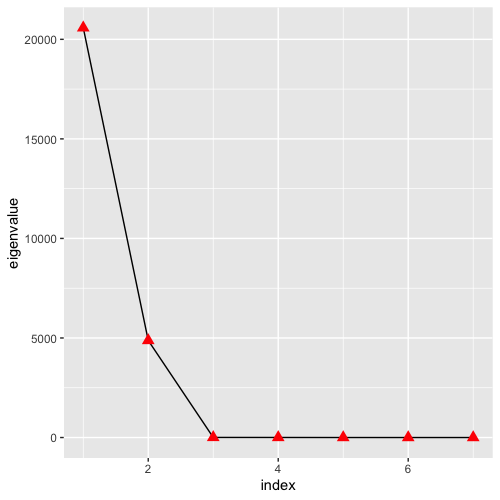
\includegraphics[width=3.0in]{9_32_S_scree.png}
\end{center}

\begin{rc}

Principal Components Analysis
Call: principal(r = X, nfactors = 2, rotate = "none", covar = TRUE, 
    scores = TRUE)
Standardized loadings (pattern matrix) based upon correlation matrix
           PC1   PC2   h2   u2 com
YrHgt     0.91 -0.05 0.84 0.16 1.0
FtFrBody  0.84  0.15 0.72 0.28 1.1
PrctFFB   0.72 -0.36 0.65 0.35 1.5
Frame     0.88  0.01 0.78 0.22 1.0
BkFat    -0.38  0.83 0.83 0.17 1.4
SaleHt    0.92  0.12 0.86 0.14 1.0
SaleWt    0.55  0.69 0.78 0.22 1.9

                       PC1  PC2
SS loadings           4.12 1.34
Proportion Var        0.59 0.19
Cumulative Var        0.59 0.78
Proportion Explained  0.76 0.24
Cumulative Proportion 0.76 1.00

Mean item complexity =  1.3
Test of the hypothesis that 2 components are sufficient.

The root mean square of the residuals (RMSR) is  0.1 
 with the empirical chi square  31.54  with prob <  0.00011 

Fit based upon off diagonal values = 0.97

\end{rc}

A rotation of the principal component factor analysis provides a different interpretation of the second factor. The second factor now seems to characterize the `fattiness' of the bull.

\begin{rc}

Principal Components Analysis
Call: principal(r = X, nfactors = 2, rotate = "varimax", covar = TRUE, 
    scores = TRUE)
Standardized loadings (pattern matrix) based upon correlation matrix
           RC1   RC2   h2   u2 com
YrHgt     0.87 -0.27 0.84 0.16 1.2
FtFrBody  0.85 -0.06 0.72 0.28 1.0
PrctFFB   0.61 -0.53 0.65 0.35 2.0
Frame     0.86 -0.21 0.78 0.22 1.1
BkFat    -0.17  0.89 0.83 0.17 1.1
SaleHt    0.92 -0.11 0.86 0.14 1.0
SaleWt    0.70  0.54 0.78 0.22 1.9

                       RC1  RC2
SS loadings           3.95 1.50
Proportion Var        0.56 0.21
Cumulative Var        0.56 0.78
Proportion Explained  0.72 0.28
Cumulative Proportion 0.72 1.00

Mean item complexity =  1.3
Test of the hypothesis that 2 components are sufficient.

The root mean square of the residuals (RMSR) is  0.1 
 with the empirical chi square  31.54  with prob <  0.00011 

Fit based upon off diagonal values = 0.97

\end{rc}

A maximum likelihood factor analysis presents a very similar first factor, but the loadings of the second factor are different from the principal components method. 

\begin{rc}

Factor Analysis using method =  ml
Call: fa(r = X, nfactors = 2, rotate = "varimax", scores = "Bartlett", 
    covar = TRUE, fm = "ml")
Unstandardized loadings (pattern matrix) based upon covariance matrix
           ML2   ML1      h2      u2   H2     U2
YrHgt     0.79  1.54 3.0e+00 5.0e-03 1.00 0.0017
FtFrBody 73.07 27.68 6.1e+03 2.5e+03 0.71 0.2895
PrctFFB   1.65  1.08 3.9e+00 6.8e+00 0.36 0.6356
Frame     0.41  0.77 7.6e-01 9.8e-02 0.89 0.1144
BkFat     0.00 -0.03 1.2e-03 6.9e-03 0.14 0.8555
SaleHt    1.36  1.24 3.4e+00 6.3e-01 0.84 0.1562
SaleWt   94.84  5.31 9.0e+03 7.8e+03 0.54 0.4645

                           ML2    ML1
SS loadings           14340.11 800.23
Proportion Var            0.56   0.03
Cumulative Var            0.56   0.59
Proportion Explained      0.95   0.05
Cumulative Proportion     0.95   1.00

 Standardized loadings (pattern matrix)
         item   ML2   ML1   h2     u2
YrHgt       1  0.45  0.89 1.00 0.0017
FtFrBody    2  0.79  0.30 0.71 0.2895
PrctFFB     3  0.51  0.33 0.36 0.6356
Frame       4  0.44  0.83 0.89 0.1144
BkFat       5 -0.01 -0.38 0.14 0.8555
SaleHt      6  0.68  0.62 0.84 0.1562
SaleWt      7  0.73  0.04 0.54 0.4645

                 ML2  ML1
SS loadings     2.28 2.21
Proportion Var  0.33 0.32
Cumulative Var  0.33 0.64
Cum. factor Var 0.51 1.00

Mean item complexity =  1.4
Test of the hypothesis that 2 factors are sufficient.

The degrees of freedom for the null model are  21  and the objective function was  25444.03 with Chi Square of  1827729
The degrees of freedom for the model are 8  and the objective function was  0.84 

The root mean square of the residuals (RMSR) is  89.32 
The df corrected root mean square of the residuals is  144.72 

The harmonic number of observations is  76 with the empirical chi square  25466809  with prob <  0 
The total number of observations was  76  with Likelihood Chi Square =  59.02  with prob <  7.3e-10

\end{rc}

The projection of the data into the two-dimensional factor space is flipped compared to the principal component method as well, though this may just be a problem with the sign of the factor two loadings. Still, based on the three graphs, each corresponding to the respective analysis above, the results from the maximum likelihood method differ drastically from the principal component method. Also, while there is an apparent outlier in the first two graphs, there is no clear outlier in the third. The spread of the data in the third plot is highly linear and does not appear to exhibit a multivariate normal spread, this may be caused by the extreme magnitude of the variance captured from the first to the second factor.

\begin{center}
	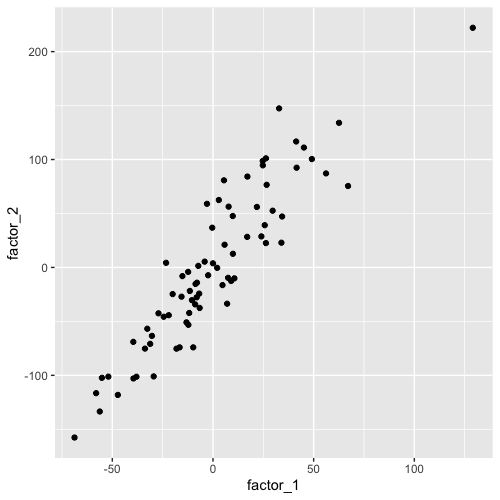
\includegraphics[width=2in]{9_32_S_fa1.png}
	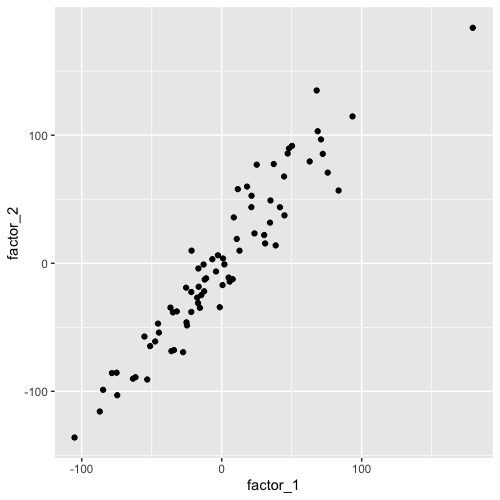
\includegraphics[width=2in]{9_32_S_fa2.png}
	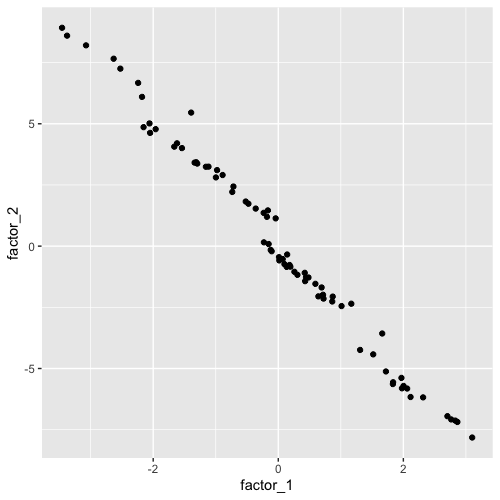
\includegraphics[width=2in]{9_32_S_fa3.png}
\end{center}

A set of factor analyses on the correlation matrix, $\mf{R}$ was also performed. Given the scree plot, it is suggested that a minimum of three factors should be used in the principal component factor analysis. However, the maximum likelihood factor analysis suggests that only two factors should be included. The loadings for the rotated principal components factor analysis for factors one and two are relatively similar to the loadings for the maximum likelihood factor analysis.

\begin{rc}

## 1. Principal Components, No Rotation
Principal Components Analysis
Call: principal(r = X, nfactors = 3, rotate = "none", covar = FALSE, 
    scores = TRUE)
Standardized loadings (pattern matrix) based upon correlation matrix
           PC1   PC2   PC3   h2    u2 com
YrHgt     0.91 -0.05 -0.36 0.96 0.035 1.3
FtFrBody  0.84  0.15  0.39 0.87 0.127 1.5
PrctFFB   0.72 -0.36  0.49 0.89 0.107 2.3
Frame     0.88  0.01 -0.39 0.93 0.072 1.4
BkFat    -0.38  0.83 -0.03 0.83 0.172 1.4
SaleHt    0.92  0.12 -0.15 0.88 0.118 1.1
SaleWt    0.55  0.69  0.22 0.83 0.170 2.1

                       PC1  PC2  PC3
SS loadings           4.12 1.34 0.74
Proportion Var        0.59 0.19 0.11
Cumulative Var        0.59 0.78 0.89
Proportion Explained  0.66 0.22 0.12
Cumulative Proportion 0.66 0.88 1.00

Mean item complexity =  1.6
Test of the hypothesis that 3 components are sufficient.

The root mean square of the residuals (RMSR) is  0.06 
 with the empirical chi square  9.84  with prob <  0.02 

Fit based upon off diagonal values = 0.99

## 2. Principal Components, Varimax Rotation
Principal Components Analysis
Call: principal(r = X, nfactors = 3, rotate = "varimax", covar = FALSE, 
    scores = TRUE)
Standardized loadings (pattern matrix) based upon correlation matrix
           RC1   RC3   RC2   h2    u2 com
YrHgt     0.94  0.27 -0.08 0.96 0.035 1.2
FtFrBody  0.45  0.79  0.21 0.87 0.127 1.7
PrctFFB   0.26  0.86 -0.29 0.89 0.107 1.4
Frame     0.94  0.22 -0.03 0.93 0.072 1.1
BkFat    -0.23 -0.34  0.81 0.83 0.172 1.5
SaleHt    0.83  0.42  0.11 0.88 0.118 1.5
SaleWt    0.35  0.43  0.72 0.83 0.170 2.1

                       RC1  RC3  RC2
SS loadings           2.90 1.97 1.33
Proportion Var        0.41 0.28 0.19
Cumulative Var        0.41 0.70 0.89
Proportion Explained  0.47 0.32 0.21
Cumulative Proportion 0.47 0.79 1.00

Mean item complexity =  1.5
Test of the hypothesis that 3 components are sufficient.

The root mean square of the residuals (RMSR) is  0.06 
 with the empirical chi square  9.84  with prob <  0.02 

Fit based upon off diagonal values = 0.99

## 3. Maximum Likelihood Factor Analysis
Factor Analysis using method =  ml
Call: fa(r = X, nfactors = 2, rotate = "varimax", scores = "Bartlett", 
    covar = FALSE, fm = "ml")
Standardized loadings (pattern matrix) based upon correlation matrix
           ML2   ML1   h2    u2 com
YrHgt     0.92  0.38 1.00 0.005 1.3
FtFrBody  0.28  0.96 1.00 0.005 1.2
PrctFFB   0.30  0.63 0.49 0.508 1.4
Frame     0.86  0.38 0.89 0.112 1.4
BkFat    -0.34 -0.08 0.12 0.879 1.1
SaleHt    0.72  0.52 0.78 0.216 1.8
SaleWt    0.18  0.53 0.31 0.689 1.2

                       ML2  ML1
SS loadings           2.42 2.16
Proportion Var        0.35 0.31
Cumulative Var        0.35 0.66
Proportion Explained  0.53 0.47
Cumulative Proportion 0.53 1.00

Mean item complexity =  1.4
Test of the hypothesis that 2 factors are sufficient.

The degrees of freedom for the null model are  21  and the objective function was  6.12 with Chi Square of  439.4
The degrees of freedom for the model are 8  and the objective function was  0.77 

The root mean square of the residuals (RMSR) is  0.11 
The df corrected root mean square of the residuals is  0.19 

The harmonic number of observations is  76 with the empirical chi square  42.04  with prob <  1.3e-06 
The total number of observations was  76  with Likelihood Chi Square =  54.34  with prob <  5.9e-09 

\end{rc}

Again, the respective plottings into the top two factors is presented below. The same problem with the `mirroring' of factor two occurs in the maximum likelihood factor analysis of the correlation matrix. However, the general spread of the data is highly similar to the principal components factor analyses. The analysis on $\mf{R}$ appears to generally be more stable given different approaches. While the factor estimates for $\mf{S}$ and $\mf{R}$ are similar, it seems preferrable to use the correlation matrix than the covariance matrix.

\begin{center}
	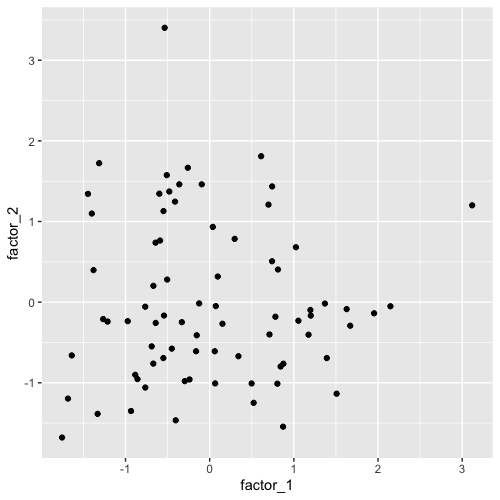
\includegraphics[width=2in]{9_32_R_fa1.png}
	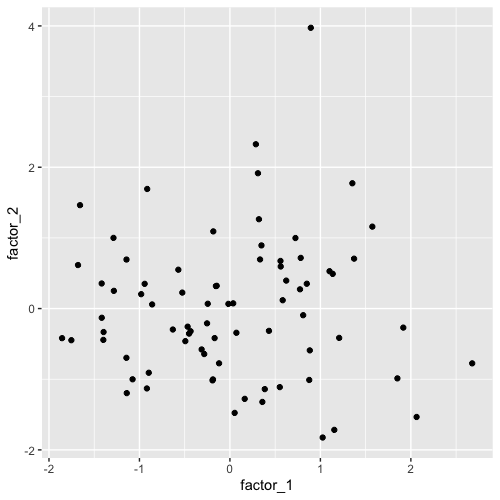
\includegraphics[width=2in]{9_32_R_fa2.png}
	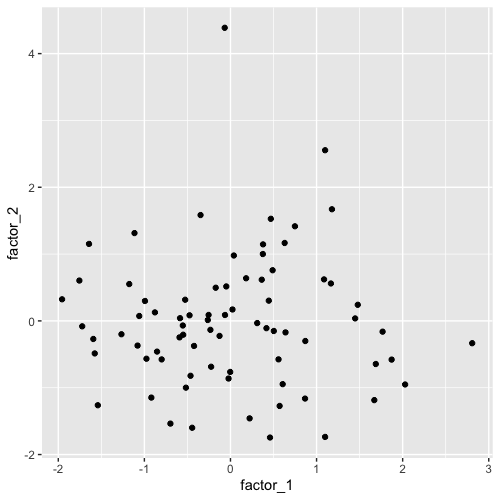
\includegraphics[width=2in]{9_32_R_fa3.png}
\end{center}

\end{document}
